AIRA is designed with a microservices architecture,
which allows for modularity, scalability, and ease of
maintenance and deployment.

\begin{figure}[H]
    \centering
    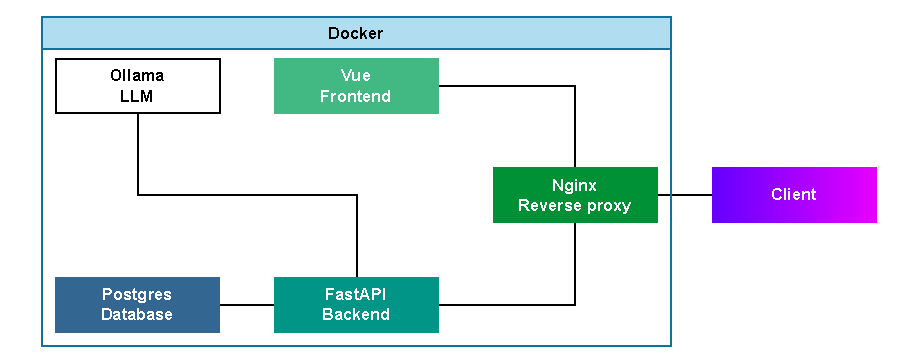
\includegraphics[width=0.9\textwidth]{figures/architecture.drawio.pdf}
    \caption{AIRA Architecture Diagram. This diagram
    illustrates the main components of AIRA and their
    interactions.}
    \label{fig:architecture}
\end{figure}

\subsection{Frontend}
We chose to implement the frontend using Vue.js, a
progressive JavaScript framework for building user
interfaces. Vue.js offers a component-based architecture,
which allows us to create reusable UI components and
manage the application state effectively. The frontend
is responsible for providing an intuitive and user-friendly
interface for users to interact with AIRA's features.

We put special attention in designing a good user experience
for both PC and mobile devices, ensuring that users can
access AIRA's functionalities seamlessly across different
platforms.

We developed the frontend using TypeScript, a
superset of JavaScript that adds static typing and
other features to the language. TypeScript helps us
catch errors early in the development process and
improves code maintainability.

The user experience is account based, meaning that users
have to create an account and log in to access AIRA's
features. This allows us to personalize the experience
for each user and store their project data securely.

\subsection{Backend}
The backend of AIRA is built using FastAPI, a modern,
fast (high-performance) web framework for building APIs
with Python. FastAPI is designed to be easy to use
and provides automatic generation of interactive API
documentation.

The backend is responsible for handling the core logic
of AIRA, including processing user requests, managing
data, and interacting with external services such as
Large Language Models (LLMs) for risk analysis and
the database for storing user and project information.

We chose FastAPI for its performance, ease of use,
and strong support for asynchronous programming, which
is essential for handling multiple concurrent requests
efficiently.
The backend exposes a RESTful API that the frontend
consumes to provide a seamless user experience.

This API requires classic client-based authentication
to be used, ensuring that only authorized users can
access their data and AIRA's features.

\subsection{Database}
AIRA uses PostgreSQL as its primary database management
system. PostgreSQL is a powerful, open-source relational
database that offers advanced features, scalability,
and reliability.

The database stores user information, project data,
identified risks and the results of their analysis.

The storage uses a docker volume to ensure data persistence,
this can be easily replaced with cloud-based storage solutions
in production environments.

\subsection{Large Language Models}
AIRA leverages Large Language Models (LLMs) to provide
its AI-powered risk analysis capabilities. We used
Ollama's local LLMs for an easy and cheap deployment.

The performance can be further improved by using
more powerful LLMs even hosted on the cloud.
This can be easily achieved because of the OpenAI API
used to interface with the LLMs, which provides a
standardized way to interact with different models.

We chose Gemma3:1B-it-qat as the default LLM for AIRA,
as it can be run locally even on laptops with no GPU
(although slowly), enabling a good testing and demo experience.
In production environments, more powerful models such as
Gemma3:12B (local) or GPT-5 (cloud) can be used to
improve the performance and accuracy of the risk analysis.

\subsection{Proxy}
To manage and route incoming requests to the appropriate
services, AIRA uses Nginx as a reverse proxy server.
Nginx is a high-performance web server that can also
be used as a load balancer and HTTP cache.

While we used HTTP, in production environments
Nginx can be easily configured to use HTTPS
with SSL/TLS certificates to ensure secure
communication between clients and the server.

We mapped the frontend to the root path ("/") and
the backend API to the "/api" path, allowing for
clear separation of concerns and easy access to
AIRA's features.
